\documentclass[12pt]{article}%
\usepackage{amsfonts}
\usepackage{fancyhdr}
\usepackage{comment}
\usepackage[a4paper, top=2.5cm, bottom=2.5cm, left=2.2cm, right=2.2cm]%
{geometry}
\usepackage{times}
\usepackage{amsmath}
\usepackage{changepage}
\usepackage{stfloats}
\usepackage{amssymb}
\usepackage{graphicx}
\usepackage{indentfirst}
\setlength{\parindent}{2em}
\setcounter{MaxMatrixCols}{30}
\newtheorem{theorem}{Theorem}
\newtheorem{acknowledgement}[theorem]{Acknowledgement}
\newtheorem{algorithm}[theorem]{Algorithm}
\newtheorem{axiom}{Axiom}
\newtheorem{case}[theorem]{Case}
\newtheorem{claim}[theorem]{Claim}
\newtheorem{conclusion}[theorem]{Conclusion}
\newtheorem{condition}[theorem]{Condition}
\newtheorem{conjecture}[theorem]{Conjecture}
\newtheorem{corollary}[theorem]{Corollary}
\newtheorem{criterion}[theorem]{Criterion}
\newtheorem{definition}[theorem]{Definition}
\newtheorem{example}[theorem]{Example}
\newtheorem{exercise}[theorem]{Exercise}
\newtheorem{lemma}[theorem]{Lemma}
\newtheorem{notation}[theorem]{Notation}
\newtheorem{problem}[theorem]{Problem}
\newtheorem{proposition}[theorem]{Proposition}
\newtheorem{remark}[theorem]{Remark}
\newtheorem{solution}[theorem]{Solution}
\newtheorem{summary}[theorem]{Summary}
\newenvironment{proof}[1][Proof]{\textbf{#1.} }{\ \rule{0.5em}{0.5em}}

\usepackage{mathtools}

\newcommand{\Q}{\mathbb{Q}}
\newcommand{\R}{\mathbb{R}}
\newcommand{\C}{\mathbb{C}}
\newcommand{\Z}{\mathbb{Z}}

\begin{document}

\title{STAT3003 Problem Sheet 4}
\author{ZHENG Weijia (William, 1155124322)}
\date{April 15, 2021}
\maketitle


\section{Q1}
\begin{figure}[htp]
    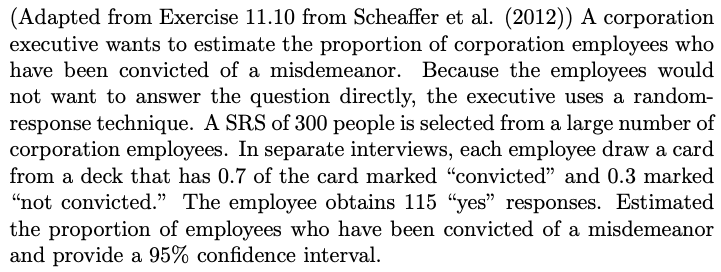
\includegraphics[width = 16cm]{img/Q1.png}
    %\caption{Section 6.1 Q8}
    %\label{fig:figure1label}
\end{figure}

\subsection*{Solution}

Let $\theta=0.7.$ And what we want to estimate is $p.$

Note that $P(Y)=115/300=\theta P(Y|C)+(1-\theta) P(Y|NC)
0.7 P(Y|C)+0.3 P(Y|NC).$

And note that $P(Y|C)=P(N|NC)=1-P(Y|NC).$

Therefore $115/300 = 0.7 P(Y|C) + 0.3 (1-P(Y|C)).$ We solve out 
$P(Y|C)=5/24.$

Hence $\hat{p}=P(Y|C)=5/24=0.2083.$

And its variance is 
$$\widehat{Var(\hat{p})}=\frac{1}{(2\theta -1)^2}(\frac{1}{n})P(Y)(1-P(Y))=4.9248\times 10^{-3}.$$

Therefore a proper 95\% C.I. for it can be 
$$(\hat{p} \pm t_{n-1,1-\frac{\alpha}{2}} \sqrt{\widehat{Var(\hat{p})}}~)=(0.2083 \pm 1.9679 \times 0.0702)=(0.2083 \pm 0.1381).$$


\newpage
\section{Q2}
\begin{figure}[htp]
    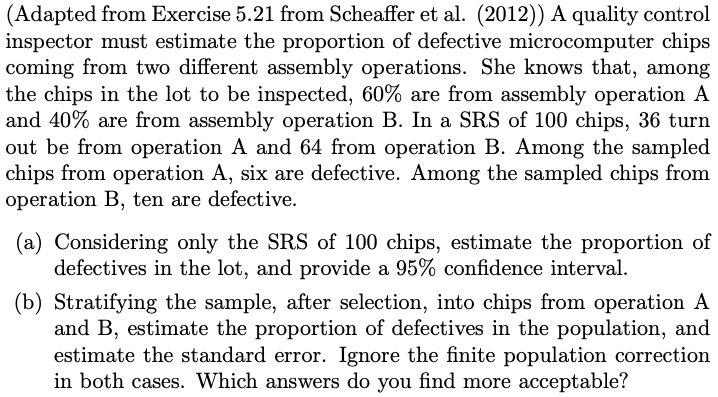
\includegraphics[width = 15cm]{img/Q2.png}
    %\caption{Section 6.1 Q8}
    %\label{fig:figure1label}
\end{figure}
\subsection*{Solution}
\subsection{(a)}
The point estimate should be $\hat{p}=\frac{6+10}{64+36}=\frac{16}{100}=0.16.$

And using $\widehat{Var(\hat{p})}=(1-\frac{n}{N})\frac{1}{n-1}\hat{p}(1-\hat{p})=1.3575\times 10^{-3}.$

Hence a proper 95\% C.I. for it should be $$(\hat{p} \pm t_{n-1,0.975}\sqrt{\widehat{Var(\hat{p})}}~)=(0.16 \pm 1.9842*0.0368)=(0.16 \pm 0.07301).$$

\subsection{(b)}
Use $\widehat{p_{pst}}=0.6*\frac{6}{36}+0.4*\frac{10}{64}=0.1625$ as the point estimate.


We stratify all the chips in the lot into 2 groups: from A and from B. 
Therefore $\hat{p_1}=\frac{6}{36}=\frac{1}{6}.$

And $\hat{p_2}=\frac{10}{64}=0.15625.$

Therefore, using $\hat{\sigma_i}^2=\frac{n_i}{n_i-1}\hat{p_i}(1-\hat{p_i}),$ one can
have $\hat{\sigma_1}^2=\frac{1}{7}.$ And $\hat{\sigma_2}^2=0.1339.$

Using the formulae 
$$\widehat{Var(\widehat{p_{pst}})}=\sum_{i=1}^{2}\frac{N-n}{nN}\frac{N_i}{N} \hat{\sigma_i}^2
+ \sum_{i=1}^2 \frac{1}{n^2}\frac{N-n}{N-1}(1-\frac{N_i}{N})\hat{\sigma_i}^2=1.4065*10^{-3}.$$

Then the s.e. is $\sqrt{1.4065*10^{-3}}=0.03750.$ 

And a 95\% C.I. for it should be $$(0.1625 \pm 1.96*0.0375) = (0.1625 \pm 0.0735).$$

I think the latter answer is more acceptable because I think the point estimate if more reasonable, 
while these two's variance are almost the same.


\newpage
\section{Q3}
\begin{figure}[htp]
    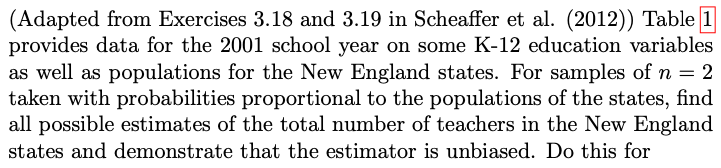
\includegraphics[width = 15cm]{img/Q3(1).png}
    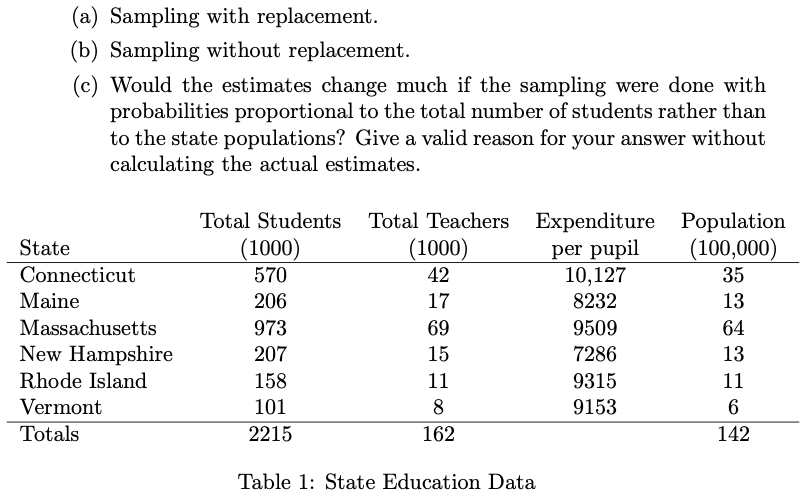
\includegraphics[width = 15cm]{img/Q3(2).png}
\end{figure}
\subsection*{Solution}



\end{document}
